\subsection{Kanal-Zeit-Eichung}
F�r eine genaue Bestimmung der Lebensdauer von Myonen ist eine exakte Zeiteichung extrem wichtig. F�r die Zeiteichung wird ein TAC, ein dual Timer und ein Oszilloskop verwendet. Der schematische Aufbau ist in Abbildung \ref{fig:kanal_zeit} zu sehen. 

\begin{figure}[H] 
	\centering
  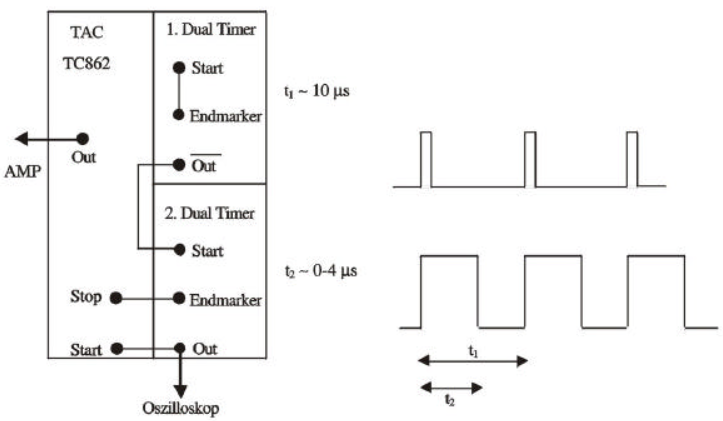
\includegraphics[scale=0.5]{kanal_zeit.png} 
	\caption{Schematischer Aufbau f�r die Kanal-Zeit-Eichung}
	\label{fig:kanal_zeit}
\end{figure}

Der dual Timer wird verwendet, um kurze Signale mit bekannter L�nge zu erzeugen. �ber die High und Lows des Signals wird der TAC gesteuert, wodurch eine Spannung in Abh�ngigkeit der L�nge des Signals erzeugt wird. Das Signal wird verst�rkt und mit dem ADC digitalisiert, damit es vom Mulit-Channel-Analyser verwertet werden kann. Durch variiren der Signall�nge lassen sich die verschiedene Kan�le ansprechen, wodurch eine Beziehung zwischen einer Zeit und einem Kanal hergestellt wird. Die Zeitintervalle werden gegen die Kan�le aufgetragen und mit Gleichung \ref{eqn:kanal} gefittet. Zum Vergleich soll zus�tzlich ein Fit mit $B = 0$ erzwungen werden. Die Parameter und Variablen des Fits sind in Tabelle \ref{tab:fit_kanal} zu sehen

\begin{align}
\label{eqn:kanal}
t = A*k+B
\end{align}

\begin{table}[H]
	\caption{Parameter des Fits}
	\label{tab:fit_kanal}
	\begin{tabular}{c|l}
	t & Zeitintervall in $\mu$s \\ 
	k & Kanal \\ 
	A & Proportionalit�tsfaktor \\ 
	B & Offset \\ 
	\end{tabular} 
\end{table}

In Abbildung \ref{fig:kanal_zeit_fit} sind die Messwerte zu sehen. F�r die Fitparameter ergaben sich dabei die Werte in Tabelle \ref{tab:fit}. Das $\chi_{red}^2$ hat ein Wert von 0,02, was einem guten Fit entspricht.

\begin{table}[H]
\centering
\caption{Fitparameter mit Fehlern und $\chi_{red}^2$}
\label{tab:fit}
\begin{tabular}{|c|c|}
\hline Paramter & Wert \\ 
\hline A & 0,002106(6) \\ 
\hline B & 0,126(19) \\ 
\hline $\chi_{red}^2$ & 0,233 \\ 
\hline 
\end{tabular} 
\end{table}

\begin{figure}[H] 
	\centering
	  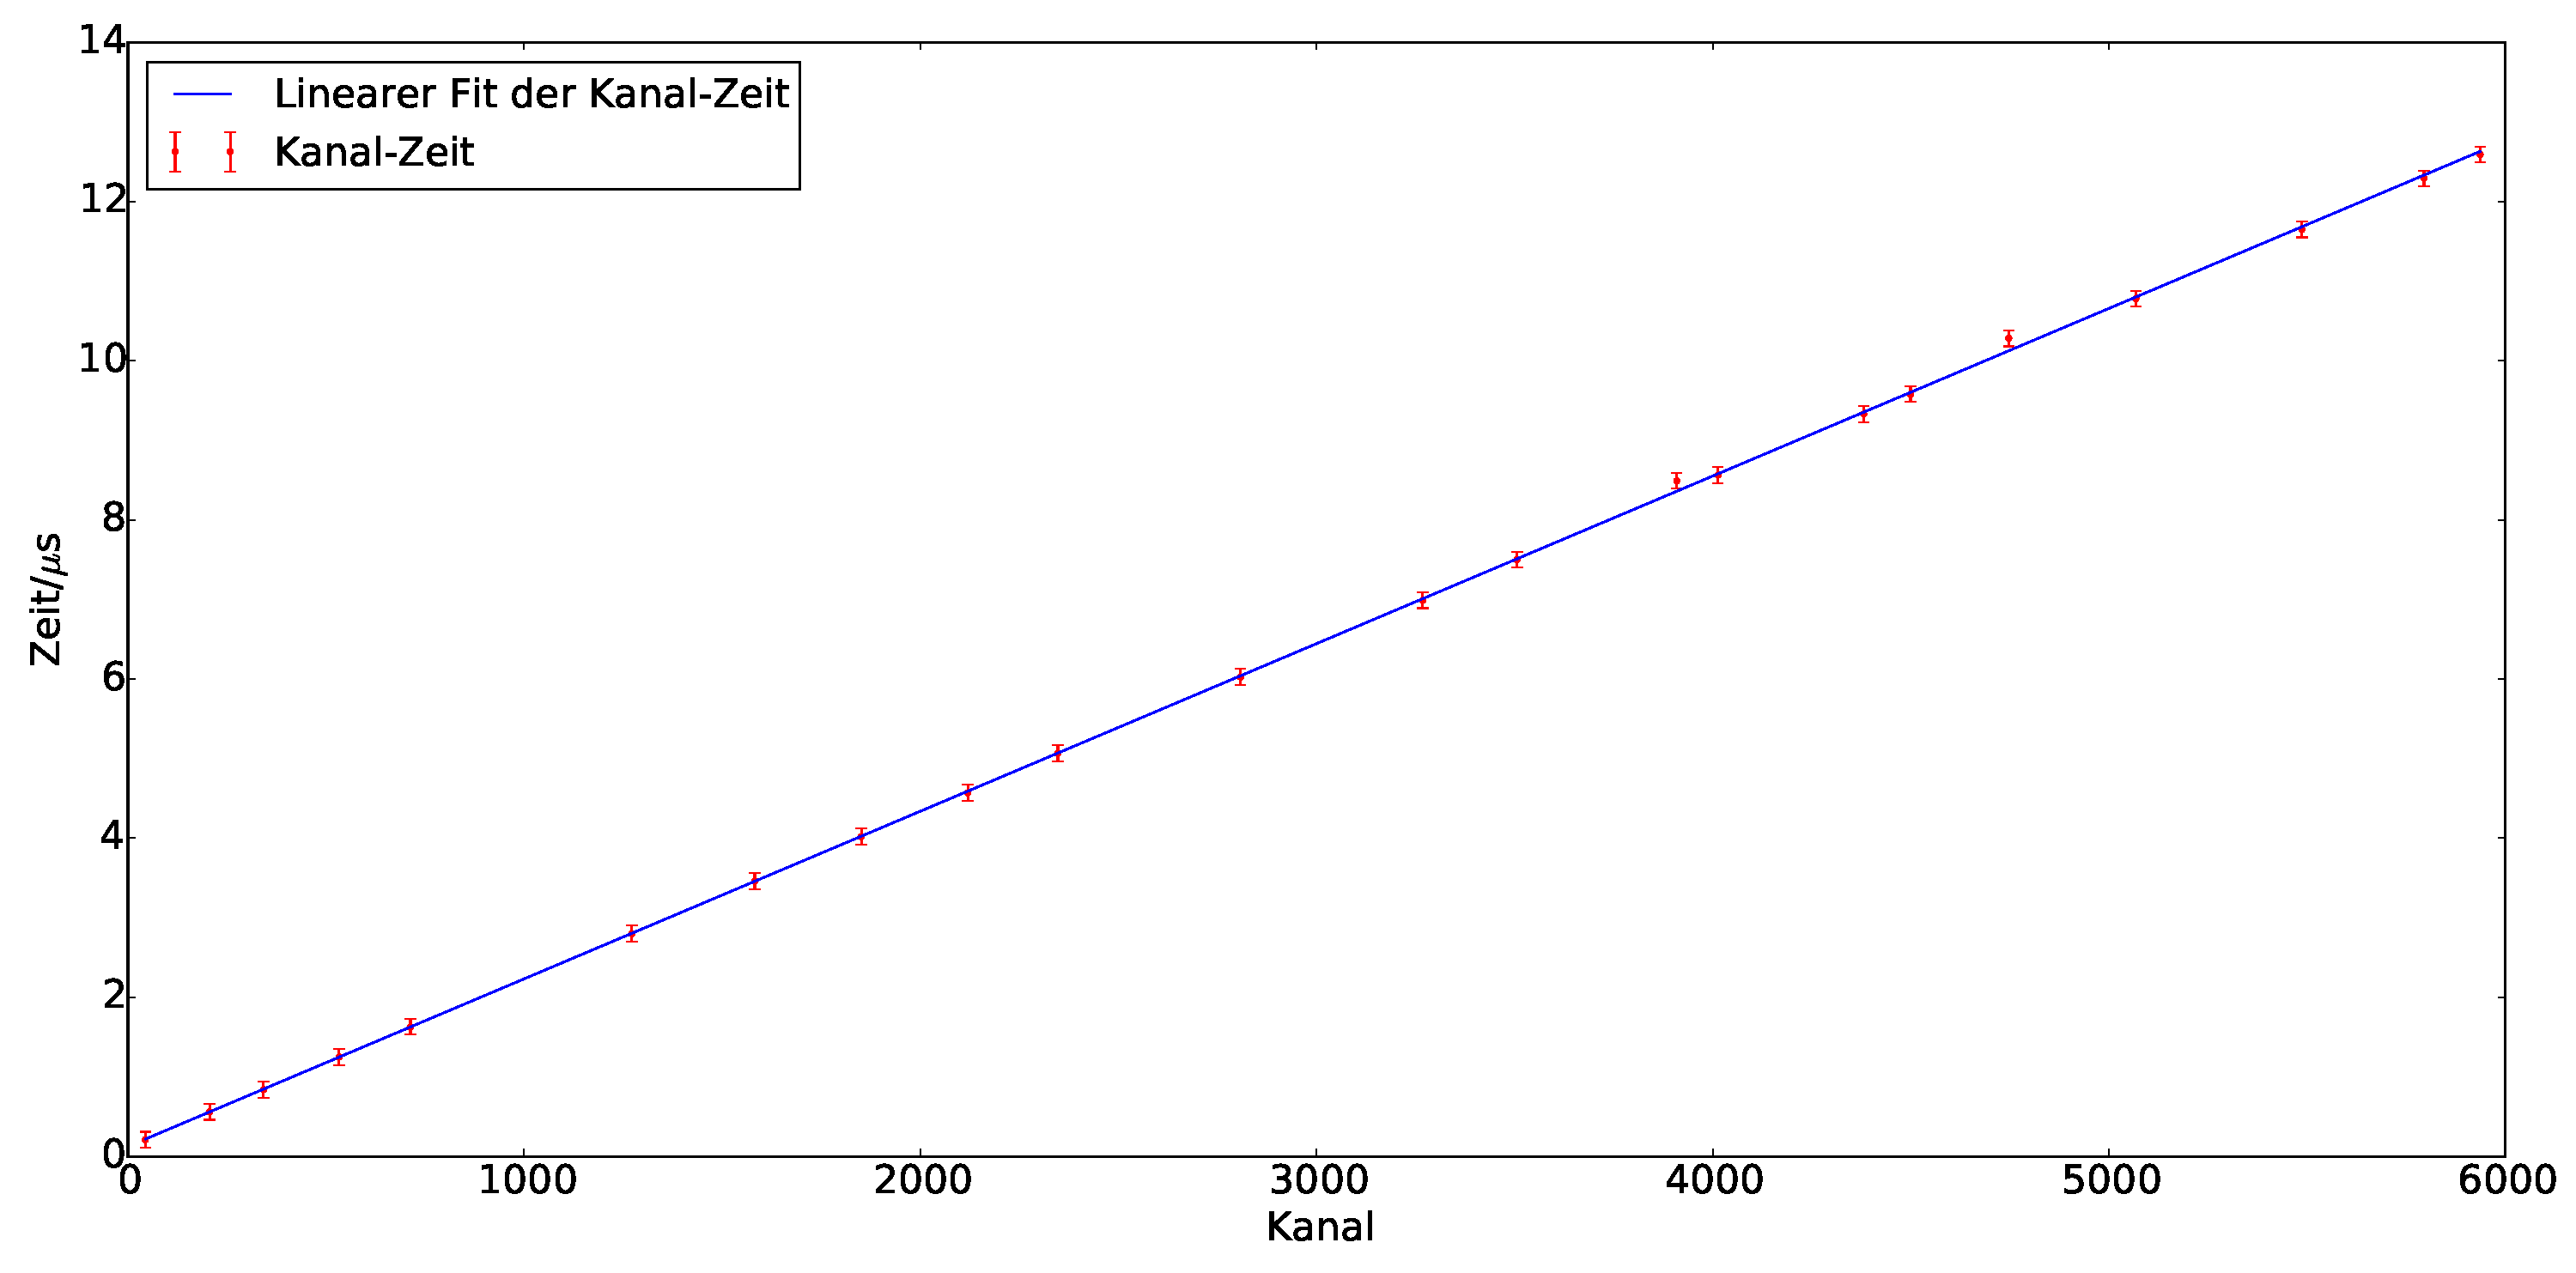
\includegraphics[scale=0.33]{kanal_zeitax+b.pdf} 
	\caption{Kanal-Zeit-Eichung}
	\label{fig:kanal_zeit_fit}
\end{figure}
Zum Vergleich sind die Fitparameter f�r $B = 0$ in Tabelle \ref{tab:fit2} zu sehen. Der Fit f�r $B = 0$ ist in Abb. \ref{fig:kanal_zeit_fit2} dargestellt.
\begin{table}[H]
\centering
\caption{Fitparameter mit Fehlern und $\chi_{red}^2$ f�r $B = 0$}
\label{tab:fit2}
\begin{tabular}{|c|c|}
\hline Paramter & Wert \\ 
\hline A & 0.002136(5) \\ 
\hline B & 0 \\ 
\hline $\chi_{red}^2$ & 0,719 \\ 
\hline 
\end{tabular} 
\end{table}
\begin{figure}[H] 
	\centering
	  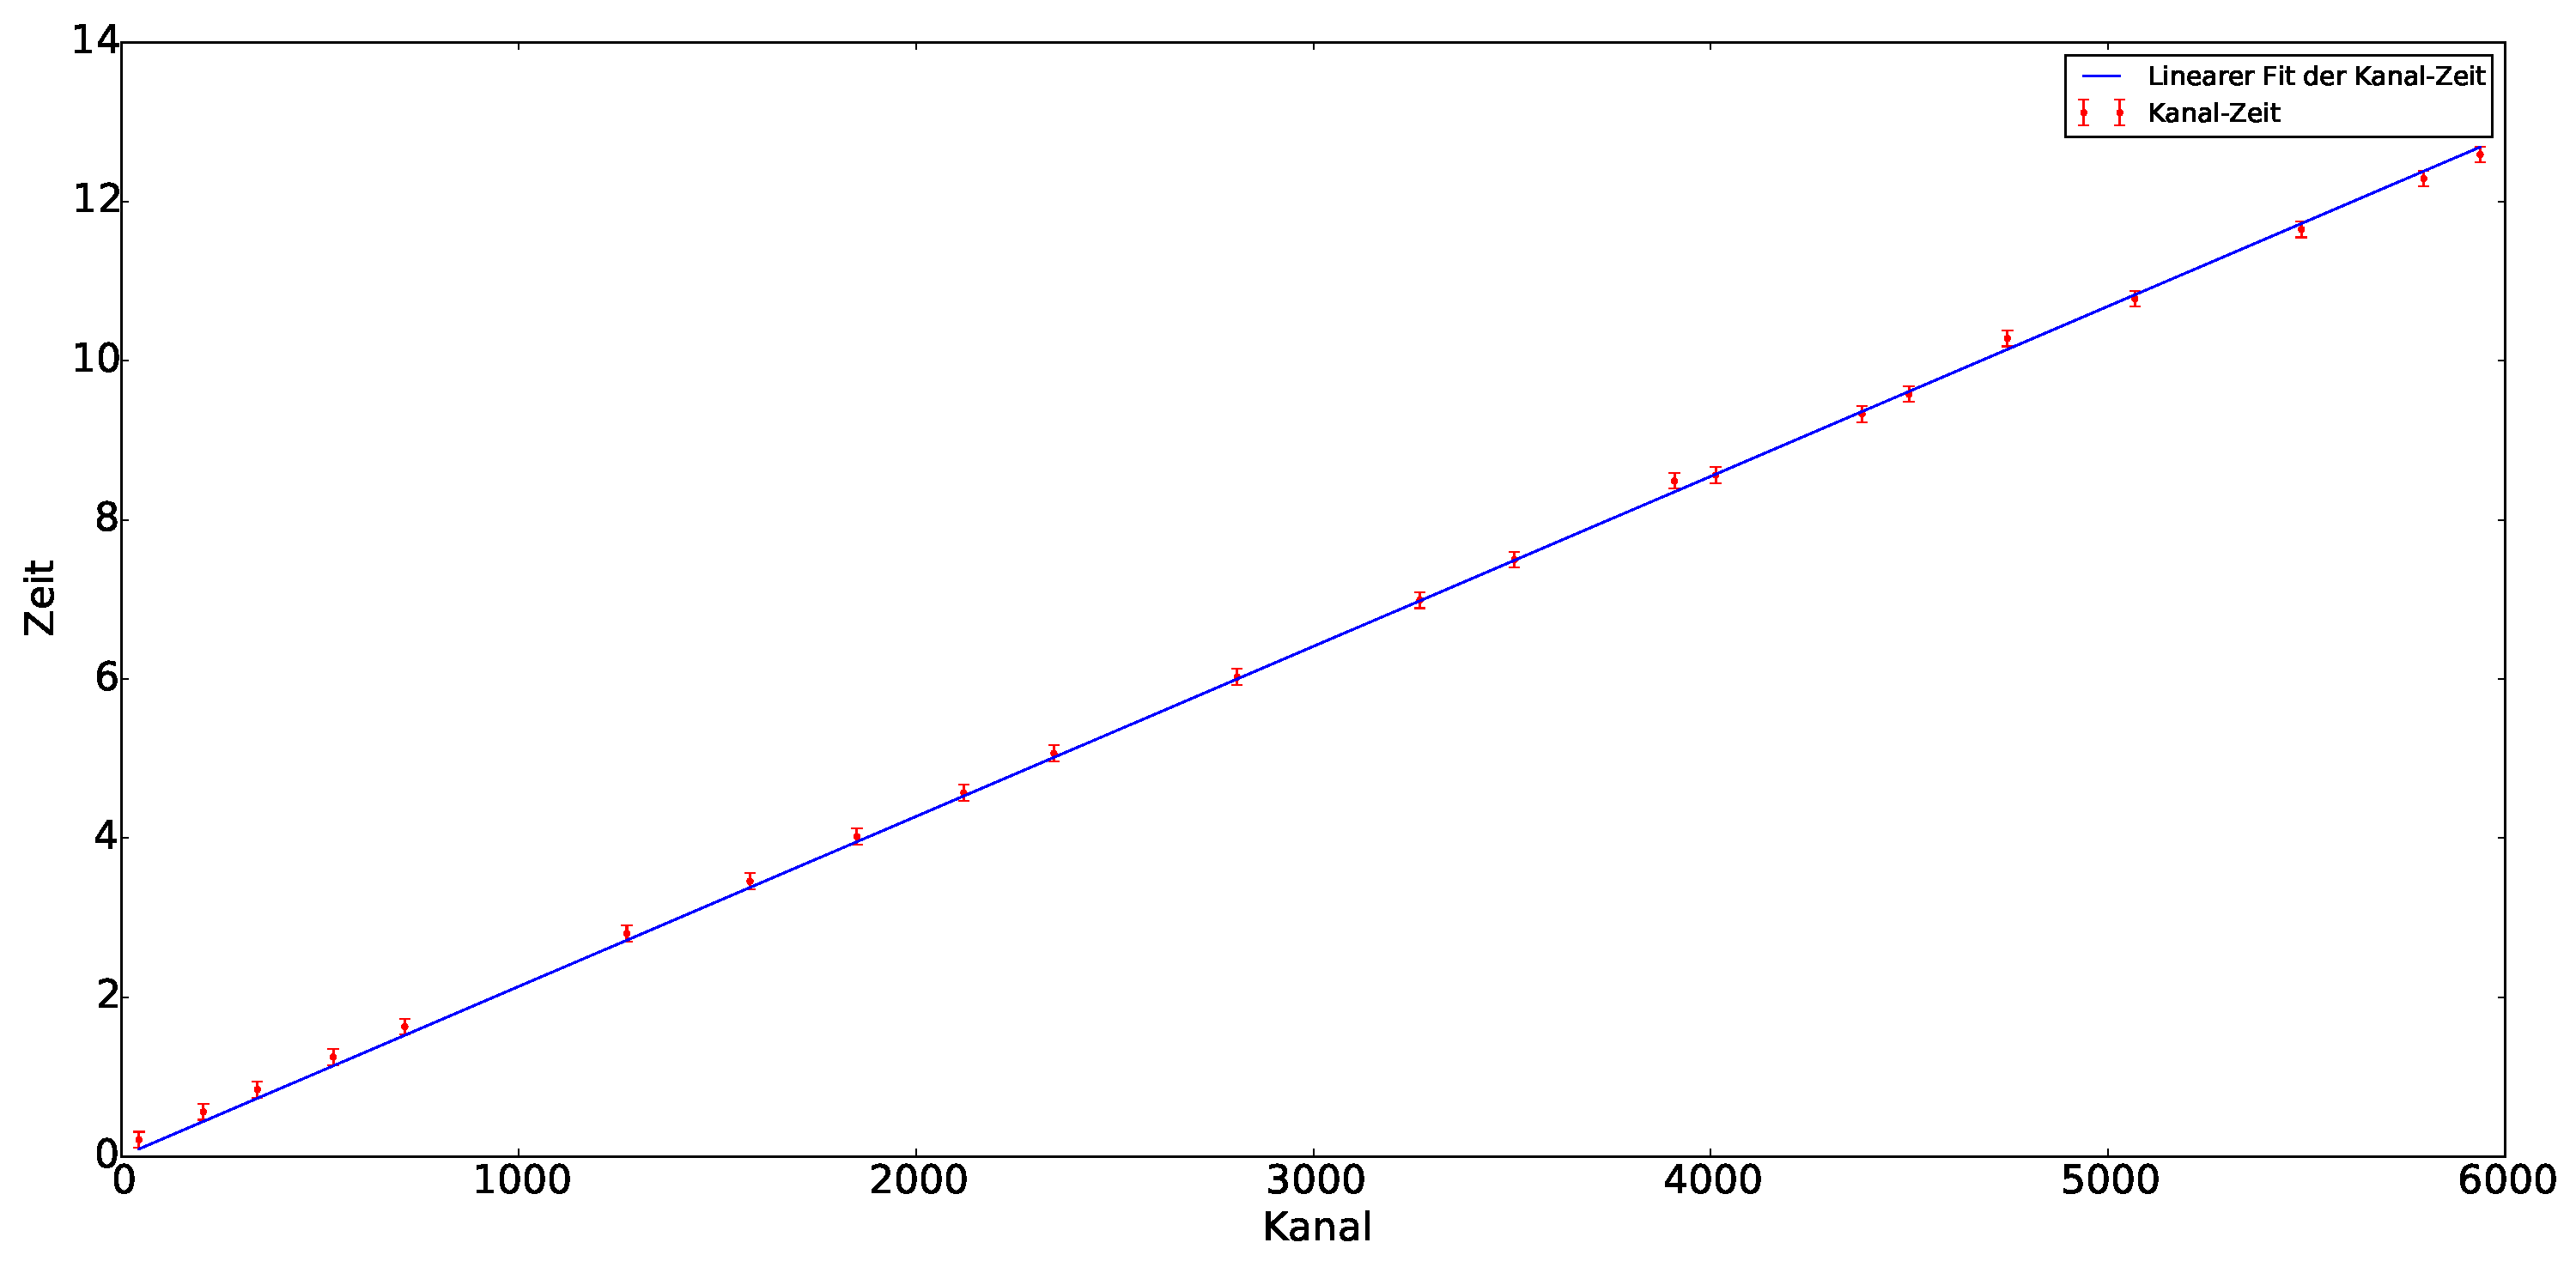
\includegraphics[scale=0.33]{kanal_zeitax.pdf} 
	\caption{Kanal-Zeit-Eichung f�r $B = 0$}
	\label{fig:kanal_zeit_fit2}
\end{figure}